%%%%%%%%%%%%%%%%%%%%%%%%%%%%%%%%%%%%%%%%%
% Beamer Presentation
% LaTeX Template
% Version 1.0 (10/11/12)
%
% This template has been downloaded from:
% http://www.LaTeXTemplates.com
%
% License:
% CC BY-NC-SA 3.0 (http://creativecommons.org/licenses/by-nc-sa/3.0/)
%
%%%%%%%%%%%%%%%%%%%%%%%%%%%%%%%%%%%%%%%%%

%----------------------------------------------------------------------------------------
%	PACKAGES AND THEMES
%----------------------------------------------------------------------------------------

\documentclass{beamer}

\mode<presentation> {

% The Beamer class comes with a number of default slide themes
% which change the colors and layouts of slides. Below this is a list
% of all the themes, uncomment each in turn to see what they look like.

%\usetheme{default}
%\usetheme{AnnArbor}
%\usetheme{Antibes}
%\usetheme{Bergen}
%\usetheme{Berkeley}
%\usetheme{Berlin}
%\usetheme{Boadilla}
%\usetheme{CambridgeUS}
%\usetheme{Copenhagen}
%\usetheme{Darmstadt}
%\usetheme{Dresden}
%\usetheme{Frankfurt}
%\usetheme{Goettingen}
%\usetheme{Hannover}
\usetheme{Ilmenau}
% \usetheme{JuanLesPins}
% \usetheme{Luebeck}
% \usetheme{Madrid}
% \usetheme{Malmoe}
% \usetheme{Marburg}
% \usetheme{Montpellier}
% \usetheme{PaloAlto}
% \usetheme{Pittsburgh}
% \usetheme{Rochester}
%\usetheme{Singapore}
%\usetheme{Szeged}
%\usetheme{Warsaw}

% As well as themes, the Beamer class has a number of color themes
% for any slide theme. Uncomment each of these in turn to see how it
% changes the colors of your current slide theme.

% \usecolortheme{albatross}
% \usecolortheme{beaver}
% \usecolortheme{beetle}
% \usecolortheme{crane}
% \usecolortheme{dolphin}
% \usecolortheme{dove}
% \usecolortheme{fly}
% \usecolortheme{lily}
% \usecolortheme{orchid}
% \usecolortheme{rose}
% \usecolortheme{seagull}
% \usecolortheme{seahorse}
% \usecolortheme{whale}
% \usecolortheme{wolverine}

%\setbeamertemplate{footline} % To remove the footer line in all slides uncomment this line
%\setbeamertemplate{footline}[page number] % To replace the footer line in all slides with a simple slide count uncomment this line

%\setbeamertemplate{navigation symbols}{} % To remove the navigation symbols from the bottom of all slides uncomment this line
}

\usepackage{bibentry}
\usepackage{graphicx} % Allows including images
\usepackage{booktabs} % Allows the use of \toprule, \midrule and \bottomrule in tables
\usepackage{bbold}

\usepackage[T1]{fontenc}
\usepackage[font=small,labelfont=bf,tableposition=top]{caption}

%----------------------------------------------------------------------------------------
%	TITLE PAGE
%----------------------------------------------------------------------------------------

\title[APSP]{Explorando a \emph{centralidade dos caminhos mínimos} em grafos.} % The short title appears at the bottom of every slide, the full title is only on the title page

\author{Ricardo Norio Miyata} % Your name
\institute[UFPR] % Your institution as it will appear on the bottom of every slide, may be shorthand to save space
{
Universidade Federal do Paraná \\ % Your institution for the title page
\medskip
\textit{rnm16@inf.ufpr.br} % Your email address
}

\date{2021} % Date, can be changed to a custom date

\graphicspath{{img/}}

\DeclareCaptionLabelFormat{andtable}{#1~#2  \&  \tablename~\thetable}

\begin{document}

\begin{frame}
\titlepage % Print the title page as the first slide
\end{frame}

\begin{frame}
\frametitle{Conteúdo da apresentação} % Table of contents slide, comment this block out to remove it
\tableofcontents % Throughout your presentation, if you choose to use \section{} and \subsection{} commands, these will automatically be printed on this slide as an overview of your presentation
\end{frame}

%----------------------------------------------------------------------------------------
%	PRESENTATION SLIDES
%----------------------------------------------------------------------------------------
\section{Objetivo}
    \begin{frame}
        \frametitle{Objetivo}
        O objetivo deste trabalho é o estudo da medida de centralidade dos caminhos mínimos.
    \end{frame}

%----------------------------------------------------------------------------------------
%	Caminhos mínimos
%----------------------------------------------------------------------------------------
\section{Fundamentação teórica}
    \subsection{Caminhos mínimos (algoritmo de \emph{Dijkstra})}
        \begin{frame}
            \frametitle{O que são caminhos mínimos}
            \begin{itemize}
                \item É o problema de encontrar um caminho entre dois vértices em um grafo de forma que a soma dos pesos de suas arestas constituintes seja minimizada.
                \item Algoritmo concebido pelo cientista da computação Edsger W. Dijkstra em 1956 e publicado três anos depois. Existem muitas variantes do algoritmo.
            \end{itemize}
        \end{frame}

        \begin{frame}
            \frametitle{Árvore de caminhos mínimos}
            \begin{itemize}
                \item Uma árvore de caminhos mínimos de um vértice $u$ é uma árvore geradora $T_u$ de $G$.
                \item Um caminho mínimo que começa na raiz de uma árvore de Dijsktra é chamado de ramo de $G$.
                \item Dado $T_u$, para cada $v \neq u$, o caminho mínimo de $u$ a $v$ é um ramo, denotado por $\mathcal{B}_u(v)$.
            \end{itemize}
        \end{frame}

        \begin{frame}
            \frametitle{Caminhos mínimos entre todos os pares de vértices (APSP)}
            \begin{itemize}
                \item O APSP, do inglês, {\it all pairs shortest paths} é o problema de calcular o comprimento mínimo entre cada par de vértices em um grafo ponderado.
            \end{itemize}
        \end{frame}

%----------------------------------------------------------------------------------------
%	Centralidade de intermediação
%----------------------------------------------------------------------------------------
    \subsection{Centralidade de intermediação (\emph{betweenness centrality})}
        \begin{frame}
            \frametitle{O que é centralidade de intermediação (\emph{betweenness centrality})}
            \begin{itemize}
                \item Uma maneira de detectar a quantidade de influência que um nó (vértice) tem sobre o fluxo de informações em um grafo.
                \item Em outras palavras, usa-se para localizar os nós que inferem ser mais "importantes".
            \end{itemize}
        \end{frame}

        \begin{frame}
            \frametitle{Ilustração: centralidade de intermediação}
            \begin{figure}
                \centering
                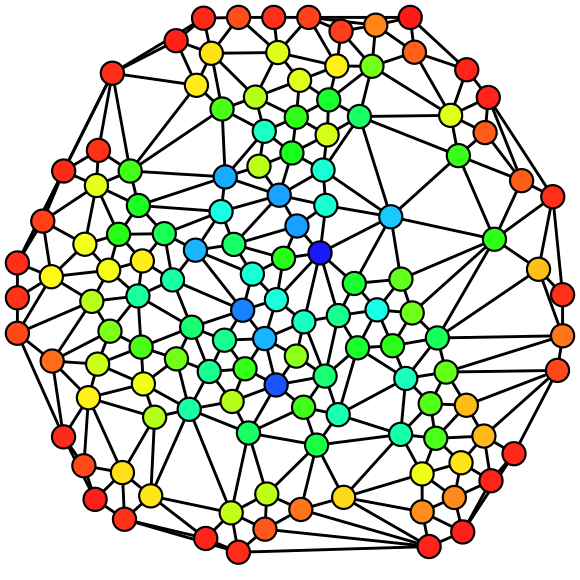
\includegraphics[scale=0.2]{graph-betweenness.png}
                \caption{Coloração de um grafo com base na centralidade da intermediação de cada vértice, do menor (vermelho) ao maior (azul).}
            \end{figure}
        \end{frame}

%----------------------------------------------------------------------------------------
%	Centralidade de caminhos mínimos
%----------------------------------------------------------------------------------------
    \subsection{Centralidade de caminhos mínimos}
        \begin{frame}
            \frametitle{Dito isto, o que é a centralidade de caminhos mínimos}
            \begin{itemize}
                \item No mesmo raciocínio, agora estamos interessados em computar a centralidade de caminhos mínimos.
                \item Em outras palavras, buscar a quantidade de influência que um caminho mínimo entre um par de vértices tem sobre o fluxo de informações em um grafo.
                \item Resumindo, caminhos mínimos com maiores valores de centralidade inferem que são mais centrais, isto é, mais "importantes".
            \end{itemize}
        \end{frame}

        \begin{frame}
            \frametitle{Centralidade de caminhos mínimos - computação}
            \begin{itemize}
                \item Calculam-se todos os caminhos mínimos possíveis entre todos os pares de vértices de um grafo.
                \item Dado um caminho mínimo, realiza-se a combinação deste com todos os demais caminhos mínimos do grafo, verificando se ele está contido como subcaminho mínimo em outro.
                \item Esta etapa é repetida para todas as combinações possíveis entre todos os pares de caminhos mínimos.
            \end{itemize}
        \end{frame}

        \begin{frame}
            \frametitle{Centralidade de caminhos mínimos - definição}
                A centralidade do caminho mínimo de um par $(u, v)$ é definida como
                \begin{align*}
                    c(u, v) &= \frac{t_{uv}}{n(n - 1)}
                \end{align*}
                onde
                \begin{align*}
                    t_{uv} &= \sum_{(a,b) \in V^2 : a \neq b} \mathbb{1}_{\tau_{uv}(\mathcal{B}_a(b))}
                \end{align*}
        \end{frame}

        \begin{frame}
            \frametitle{Centralidade de caminhos mínimos - definição}
            Explicando: A função $\mathbb{1}_{\tau_{uv}(\mathcal{B}_a(b))}$ retorna 1 se houver algum caminho mínimo de $u$ a $v$ como subcaminho do ramo $\mathcal{B}_a(b) \in S (T_a)$ (e 0 caso contrário). Intuitivamente falando, um par $(u, v)$ tem alta centralidade de caminho mínimo se o caminho mínimo canônico $p_{uv} \in S(T_u)$ (e $S(T_v)$) é um subcaminho de um grande número de caminhos canônicos mínimos em $S(G)$.
        \end{frame}

%----------------------------------------------------------------------------------------
%	Arquitetura dos grafos de entrada
%----------------------------------------------------------------------------------------
\section{Método e Resultados}
    \subsection{Arquitetura dos grafos de entrada}
        \begin{frame}
            \frametitle{Relembrando o objetivo}
            O objetivo deste trabalho é o estudo da medida de centralidade dos caminhos mínimos.
        \end{frame}

        \begin{frame}
            \frametitle{Grafos de entrada}
            Para a computação e análise dos valores de centralidade dos caminhos mínimos, foram usados 3 tipos de grafos:
            \begin{itemize}
                \item Implementado manualmente, um grafo simples, com 5 vértices;
                \item Representação do clube de karate de Zachary;
                \item Uma rede de jogos de futebol americano.
            \end{itemize}
        \end{frame}

        \begin{frame}
            \frametitle{Grafo simples}
            \begin{figure}
                \centering
                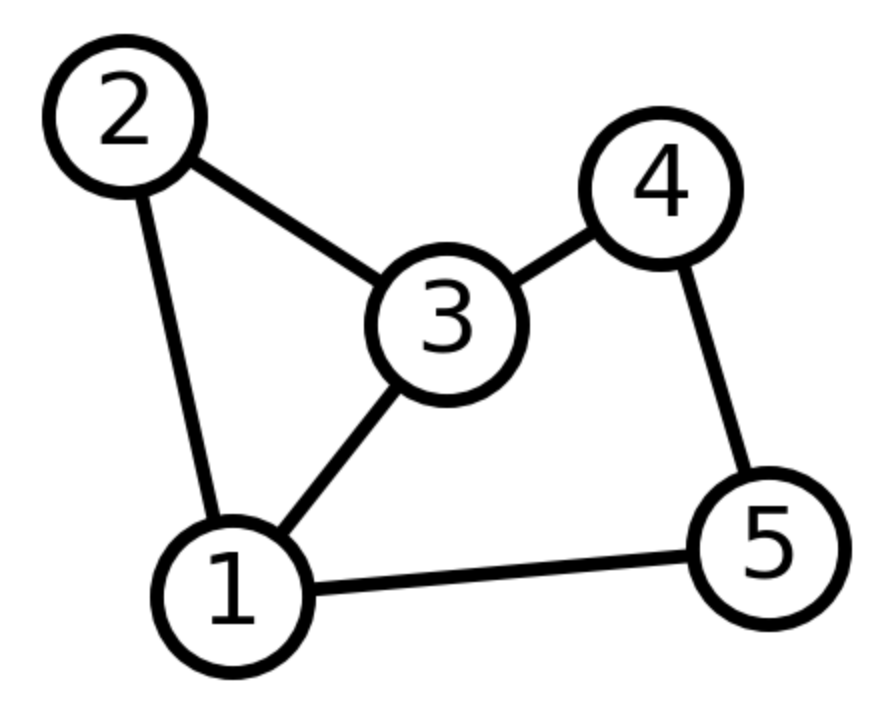
\includegraphics[scale=0.35]{simple-graph.png}
                \caption{Grafo simples, implementado manualmente, é conexo e possui 5 vértices.}
            \end{figure}
        \end{frame}

        \begin{frame}
            \frametitle{Clube de karate de Zachary}
            \begin{figure}
                \centering
                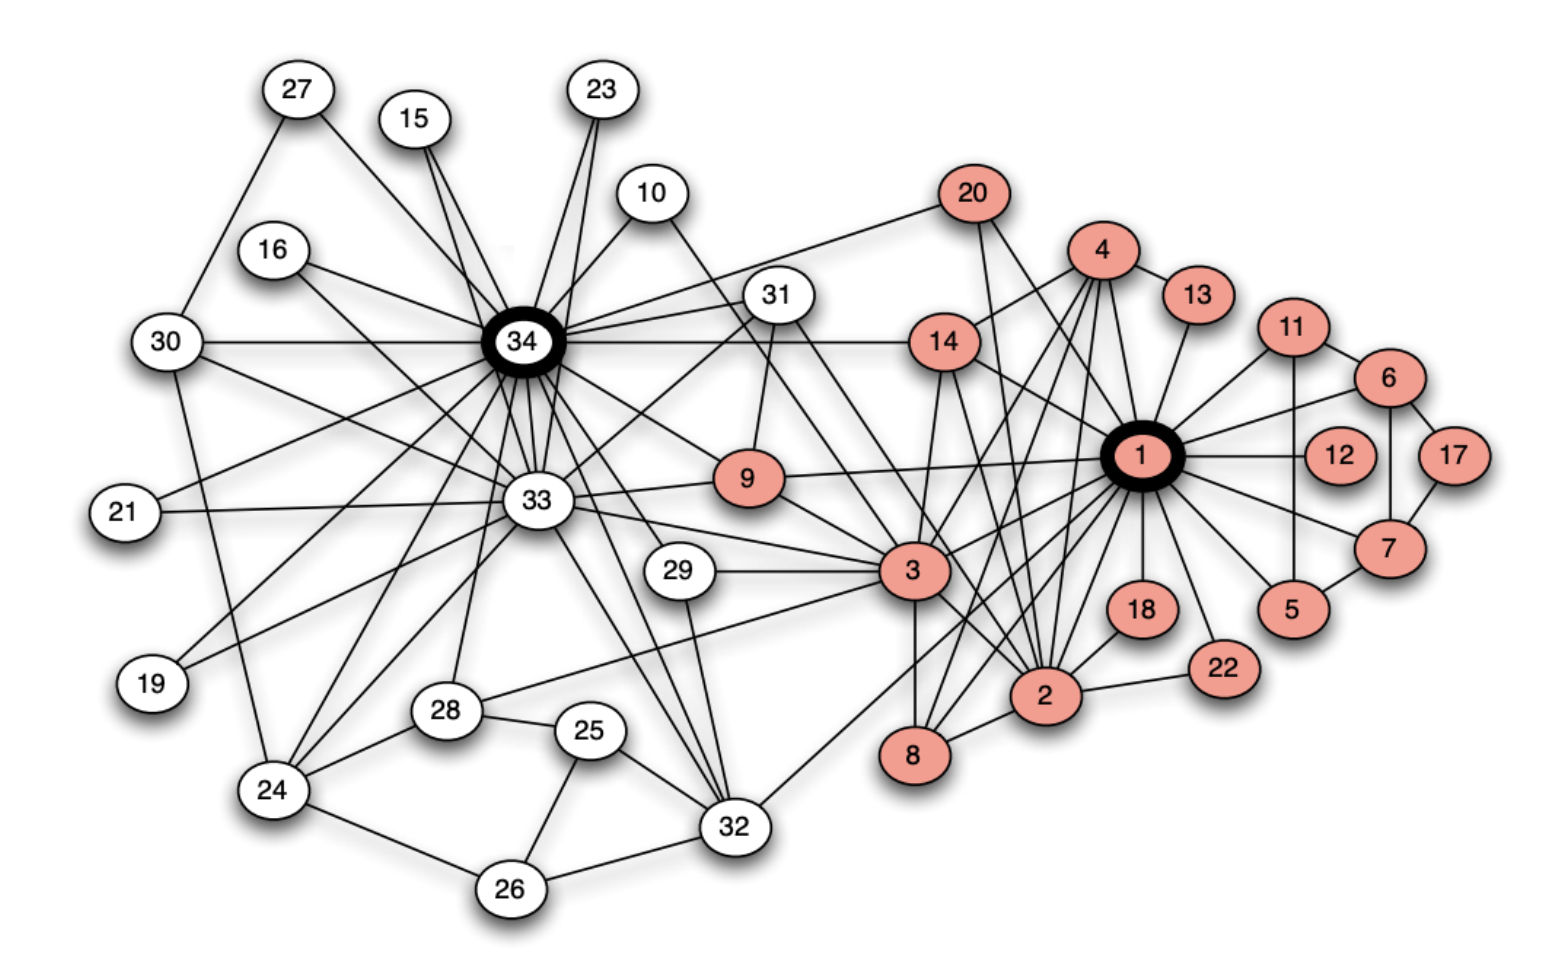
\includegraphics[scale=0.3]{karate-club-network.png}
                \caption{Grafo fortemente subdivido em duas partes.}
            \end{figure}
        \end{frame}

        \begin{frame}
            \frametitle{Rede de jogos de futebol americano}
            \begin{figure}
                \centering
                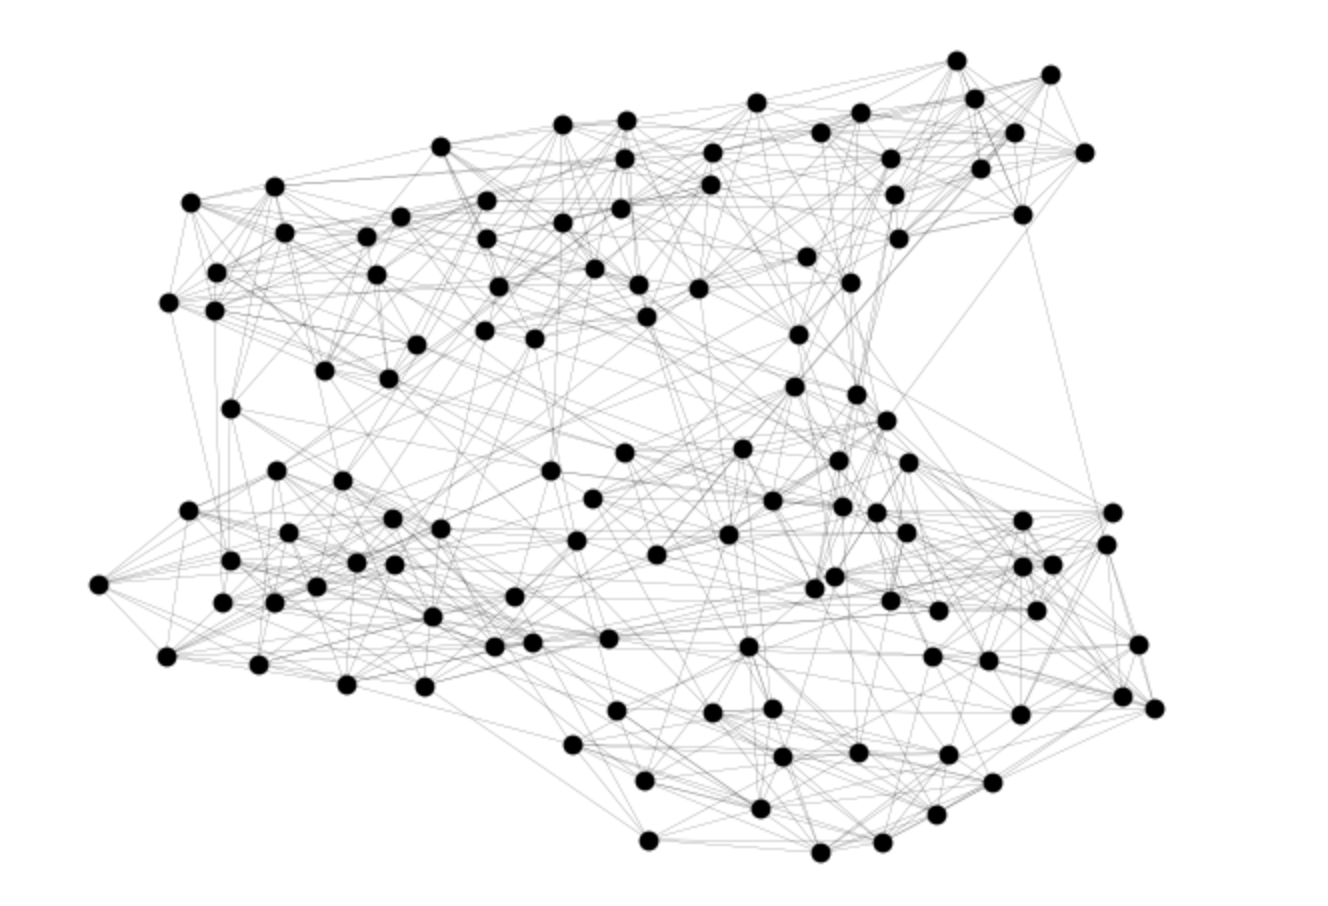
\includegraphics[scale=0.3]{american-football.png}
                \caption{Rede de jogos de futebol americano entre faculdades da Divisão IA durante a temporada regular, outono de 2000.}
            \end{figure}
        \end{frame}

%----------------------------------------------------------------------------------------
%	Fluxo da computação
%----------------------------------------------------------------------------------------
    \subsection{Fluxo da computação}
        \begin{frame}
            \frametitle{Fluxo da computação}
            \begin{figure}
                \centering
                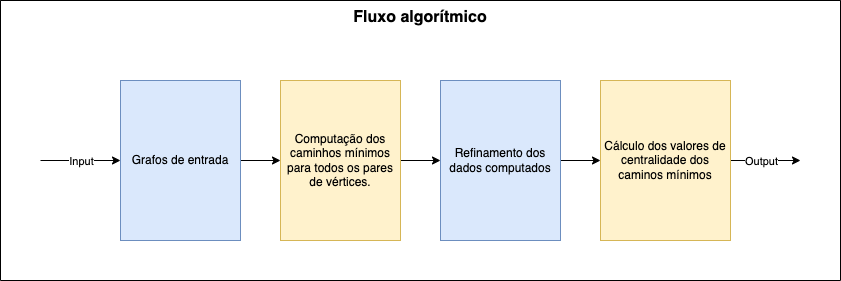
\includegraphics[scale=0.3]{algorithmic-flow.png}
                \caption{As caixas amarelas representam computação matemática, enquanto que as azuis representam computações de leitura, escrita e refinamento (sem cálculos).}
            \end{figure}
        \end{frame}

%----------------------------------------------------------------------------------------
%	Análise dos resultados
%----------------------------------------------------------------------------------------
    \subsection{Resultados}
        \begin{frame}
            \frametitle{Tabela com os valores de centralidade dos caminhos minimos}
            \begin{minipage}{\textwidth}
                \begin{minipage}[b]{0.49\textwidth}
                    \begin{figure}
                        \centering
                        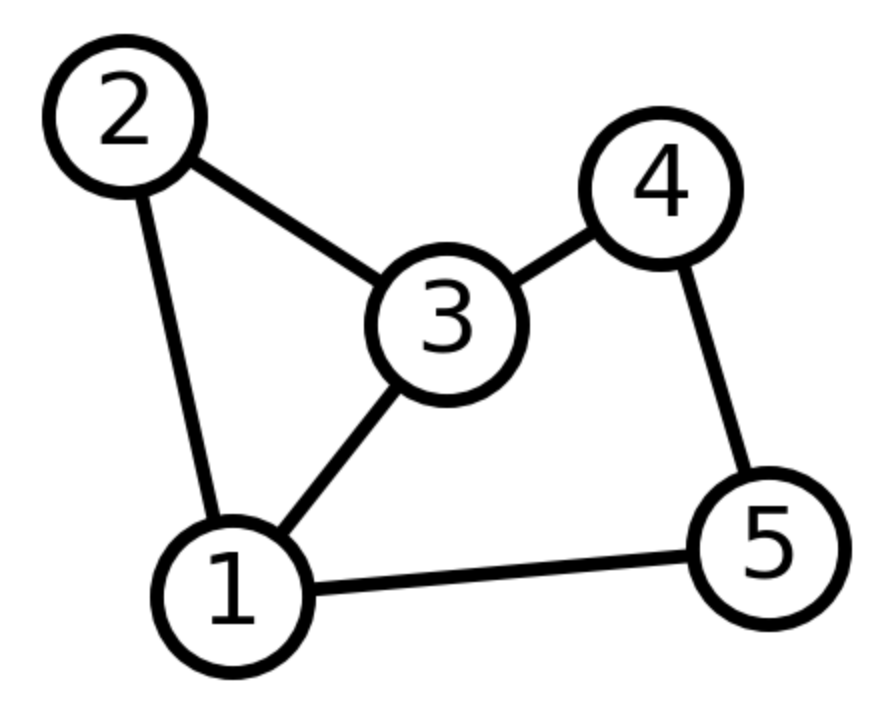
\includegraphics[scale=0.3]{simple-graph.png}
                    \end{figure}
                    \captionof{figure}{Grafo simples, com 5 vértices.}
                \end{minipage}
                \hfill
                \begin{minipage}[b]{0.49\textwidth}
                    \centering
                    \resizebox{1.8cm}{!}{
                        \begin{tabular}{|c|c|}
                            \hline
                            \textbf{Path} & \textbf{Centrality} \\ \hline
                            {[}1, 2{]}    & {[}0.050{]}         \\
                            {[}1, 3{]}    & {[}0.075{]}         \\
                            {[}1, 5{]}    & {[}0.075{]}         \\
                            {[}1, 3, 4{]} & {[}0.016{]}         \\
                            {[}2, 1{]}    & {[}0.050{]}         \\
                            {[}2, 3{]}    & {[}0.050{]}         \\
                            {[}2, 1, 5{]} & {[}0.016{]}         \\
                            {[}2, 3, 4{]} & {[}0.016{]}         \\
                            {[}3, 1{]}    & {[}0.075{]}         \\
                            {[}3, 2{]}    & {[}0.050{]}         \\
                            {[}3, 4{]}    & {[}0.075{]}         \\
                            {[}3, 1, 5{]} & {[}0.016{]}         \\
                            {[}5, 1{]}    & {[}0.075{]}         \\
                            {[}5, 4{]}    & {[}0.025{]}         \\
                            {[}5, 1, 2{]} & {[}0.016{]}         \\
                            {[}5, 1, 3{]} & {[}0.016{]}         \\
                            {[}4, 3{]}    & {[}0.075{]}         \\
                            {[}4, 5{]}    & {[}0.025{]}         \\
                            {[}4, 3, 1{]} & {[}0.016{]}         \\
                            {[}4, 3, 2{]} & {[}0.016{]}         \\ \hline
                        \end{tabular}
                    }
                    \captionof{table}{Centralidade dos caminhos mínimos do grafo simples.}
                \end{minipage}
            \end{minipage}
        \end{frame}

        \begin{frame}
            \frametitle{Distribuição dos valores de centralidade, normalizados, dos caminhos mínimos.}
            \begin{minipage}{\textwidth}
                \begin{minipage}[b]{0.49\textwidth}
                    \begin{figure}
                        \centering
                        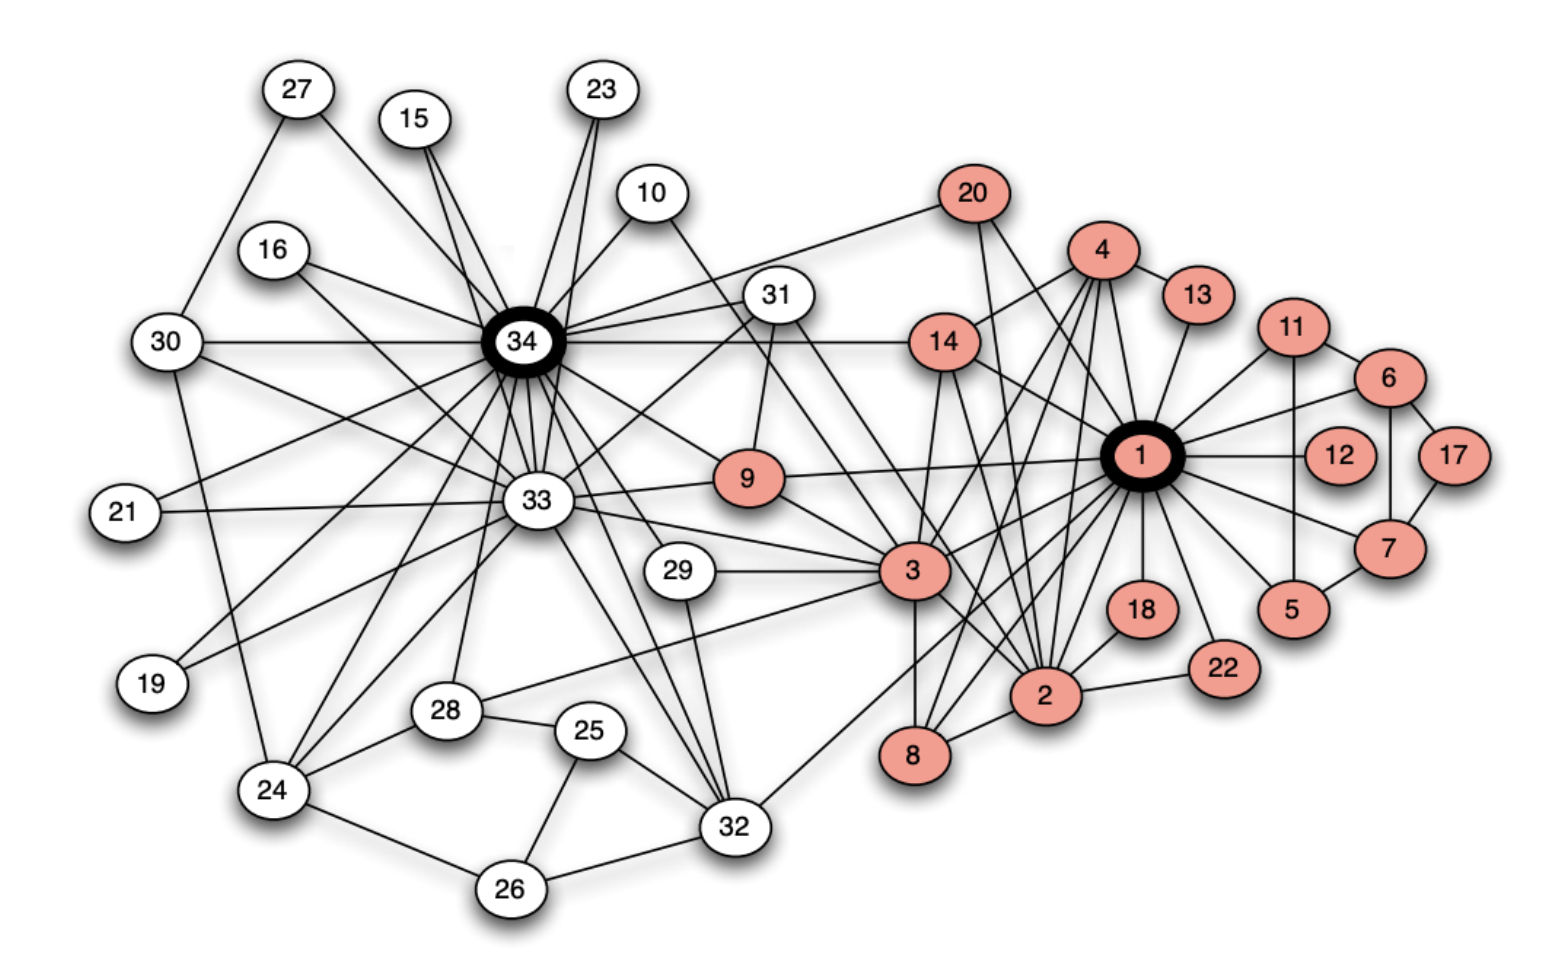
\includegraphics[scale=0.2]{karate-club-network.png}
                    \end{figure}
                    \captionof{figure}{Clube de karatê de Zachary.}
                \end{minipage}
                \hfill
                \begin{minipage}[b]{0.49\textwidth}
                    \begin{figure}
                        \centering
                        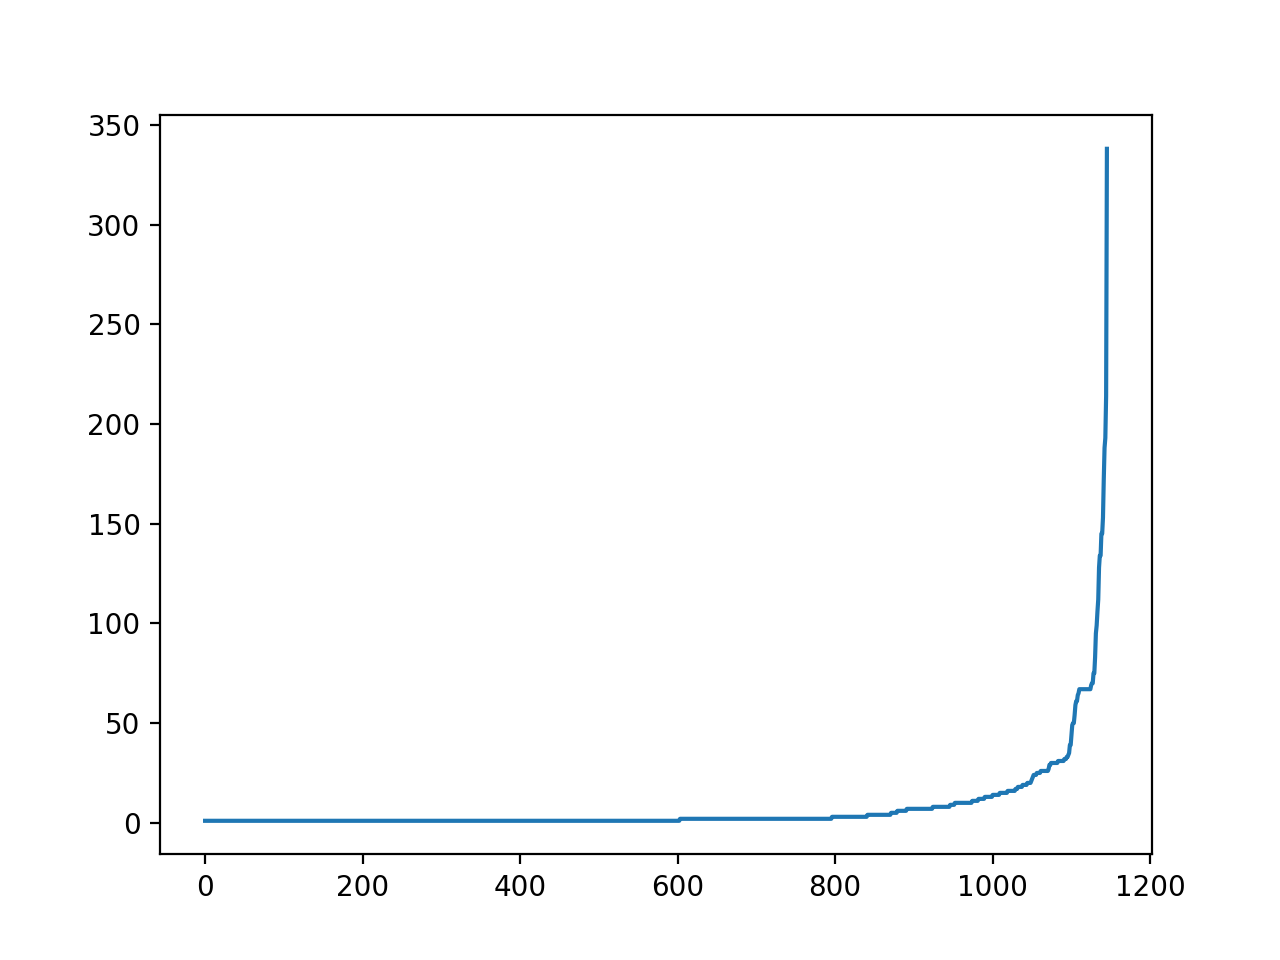
\includegraphics[scale=0.3]{short_path_centrality_ex2.png}
                    \end{figure}
                    \captionof{figure}{Representação gráfica.}
                \end{minipage}
            \end{minipage}
        \end{frame}

        \begin{frame}
            \frametitle{Distribuição dos valores de centralidade, não normalizados e na escala logarítmica, dos caminhos mínimos.}
            \begin{minipage}{\textwidth}
                \begin{minipage}[b]{0.49\textwidth}
                    \begin{figure}
                        \centering
                        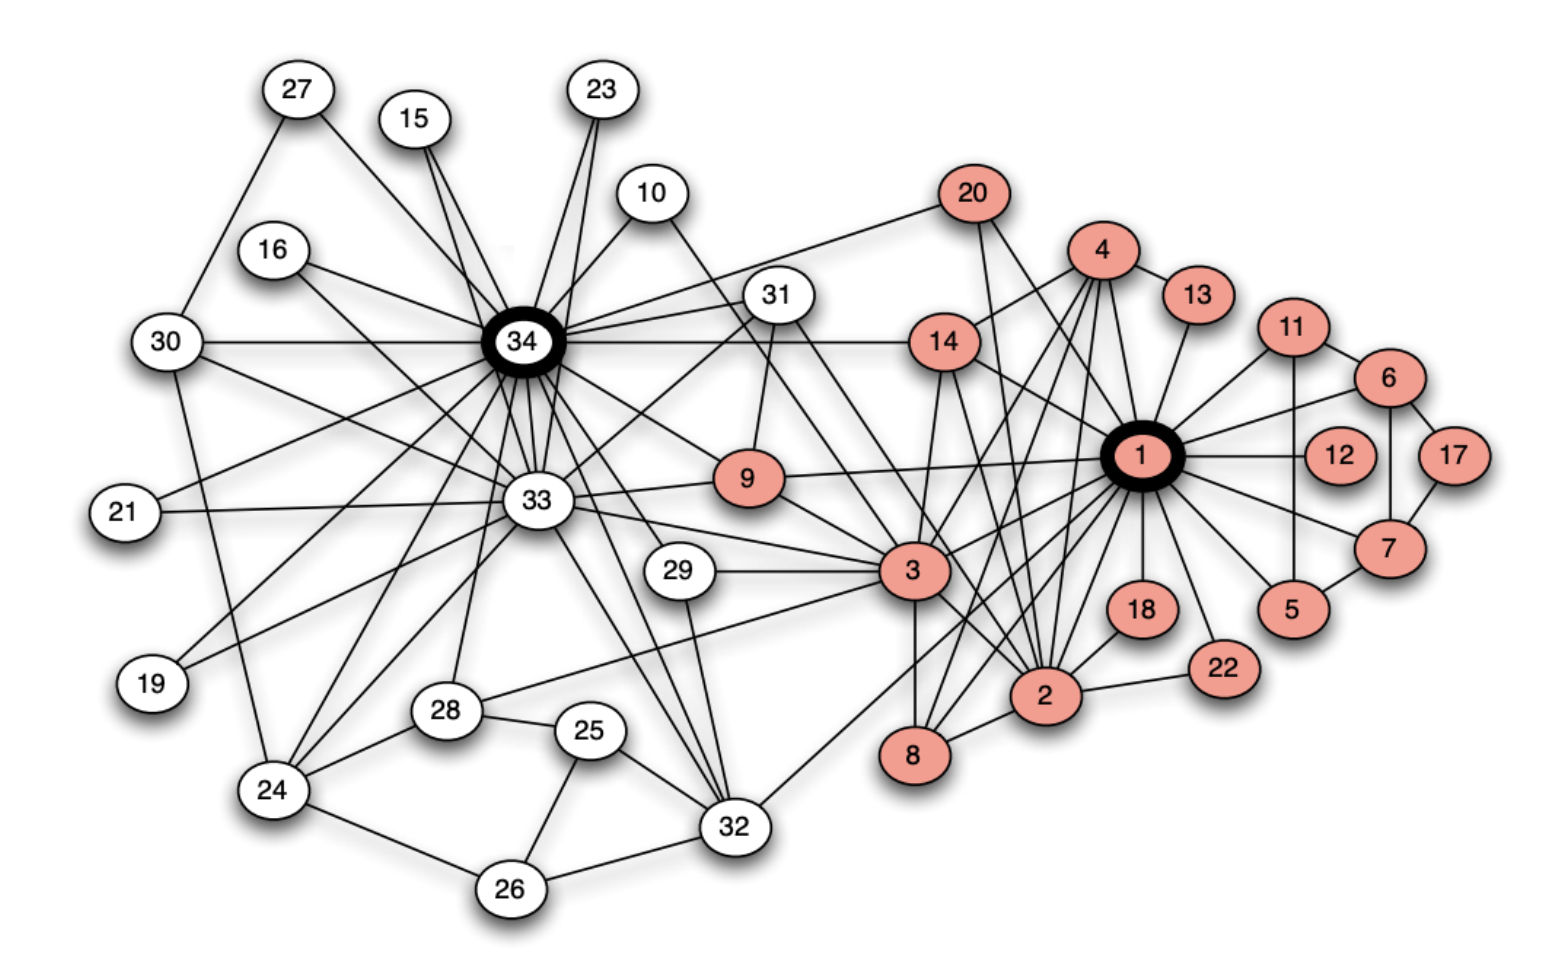
\includegraphics[scale=0.2]{karate-club-network.png}
                    \end{figure}
                    \captionof{figure}{Clube de karatê de Zachary.}
                \end{minipage}
                \hfill
                \begin{minipage}[b]{0.49\textwidth}
                    \begin{figure}
                        \centering
                        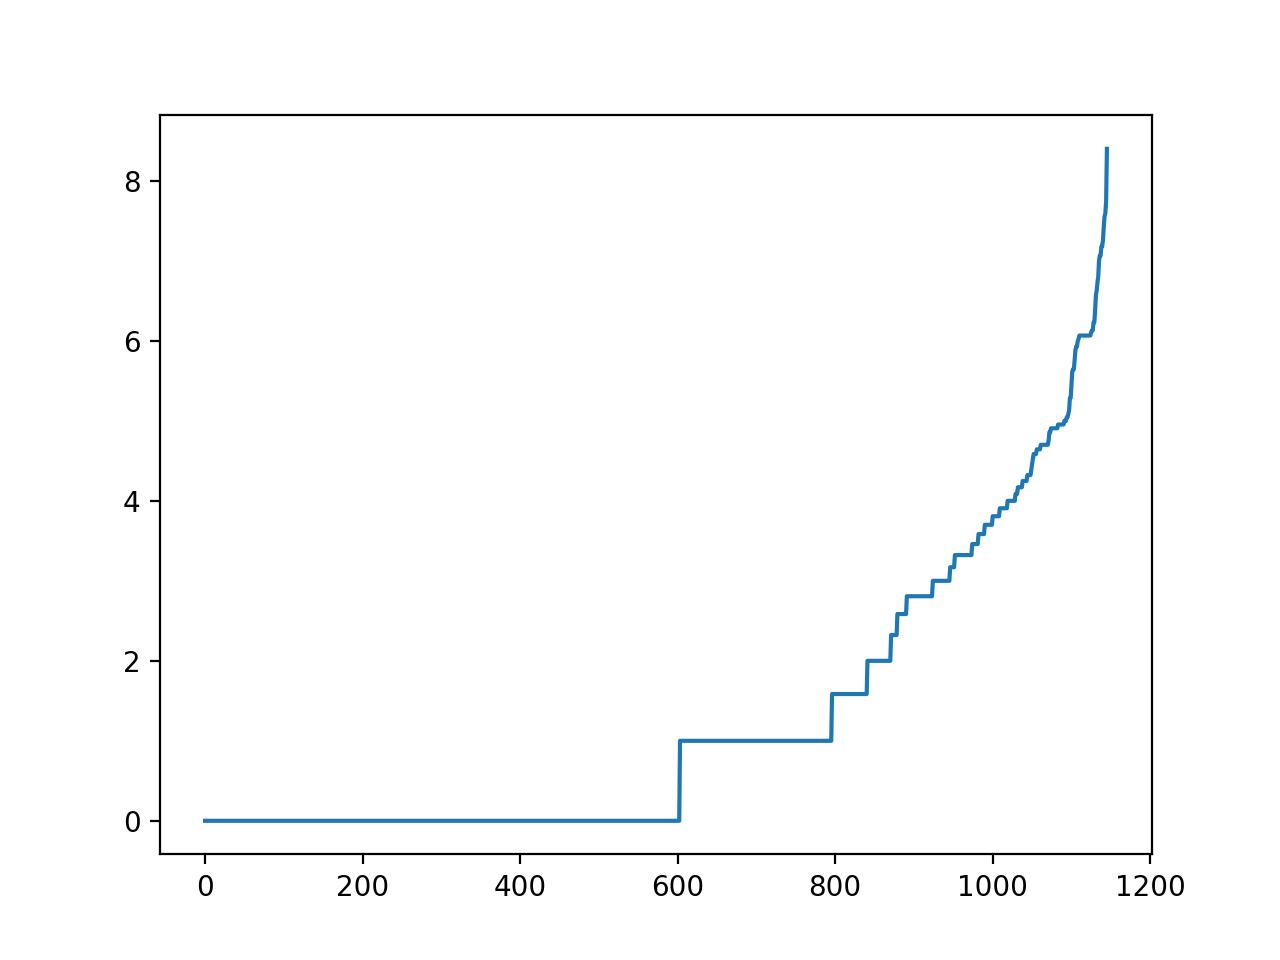
\includegraphics[scale=0.3]{short_path_centrality_ex2_log.png}
                    \end{figure}
                    \captionof{figure}{Representação gráfica.}
                \end{minipage}
            \end{minipage}
        \end{frame}

        \begin{frame}
            \frametitle{Distribuição dos valores de centralidade, normalizados, dos caminhos mínimos.}
            \begin{minipage}{\textwidth}
                \begin{minipage}[b]{0.49\textwidth}
                    \begin{figure}
                        \centering
                        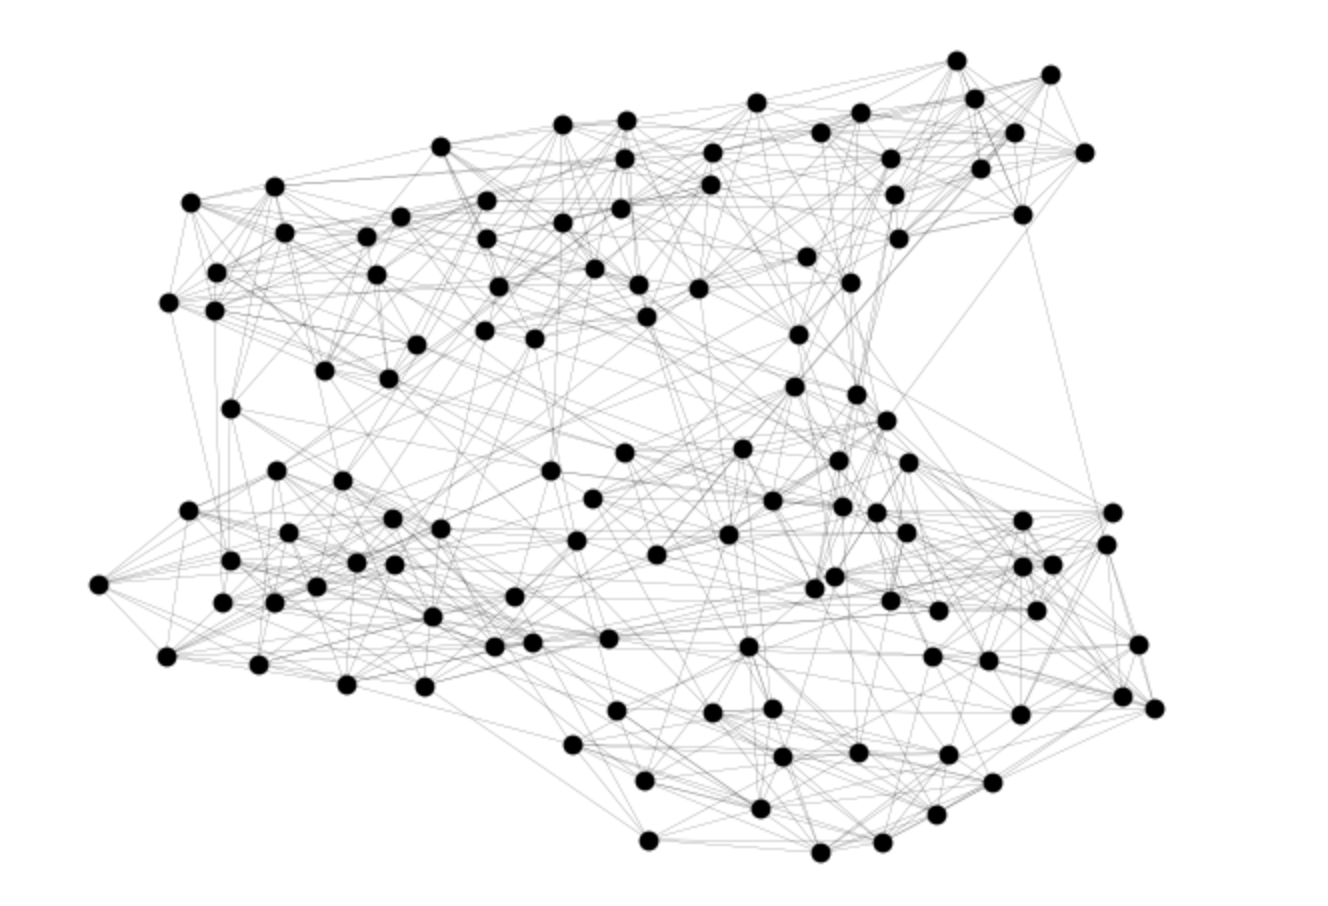
\includegraphics[scale=0.25]{american-football.png}
                    \end{figure}
                    \captionof{figure}{Clube de karatê de Zachary.}
                \end{minipage}
                \hfill
                \begin{minipage}[b]{0.49\textwidth}
                    \begin{figure}
                        \centering
                        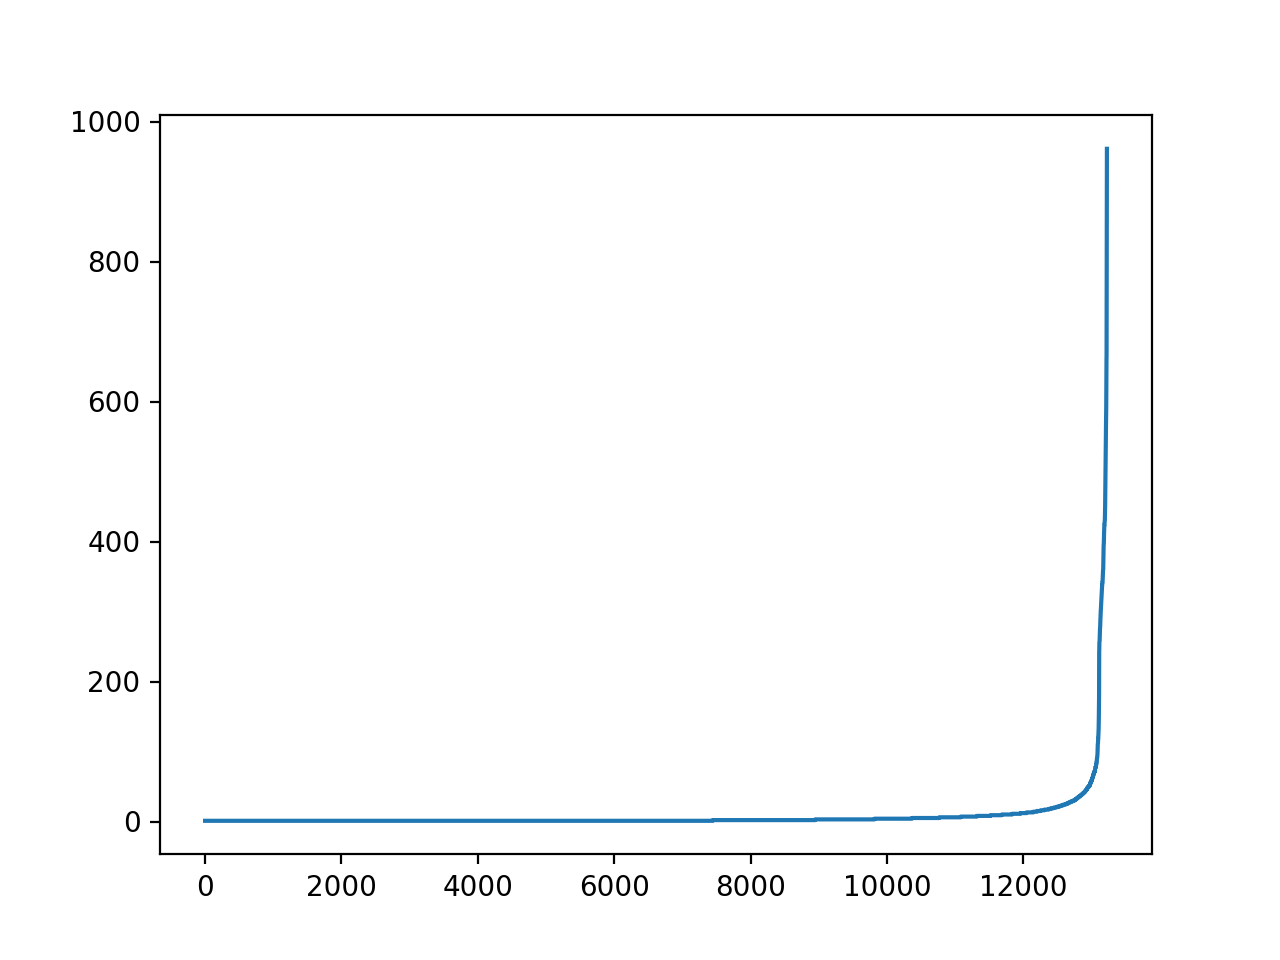
\includegraphics[scale=0.3]{short_path_centrality_ex3.png}
                    \end{figure}
                    \captionof{figure}{Representação gráfica.}
                \end{minipage}
            \end{minipage}
        \end{frame}

        \begin{frame}
            \frametitle{Distribuição dos valores de centralidade, não normalizados e na escala logarítmica, dos caminhos mínimos.}
            \begin{minipage}{\textwidth}
                \begin{minipage}[b]{0.49\textwidth}
                    \begin{figure}
                        \centering
                        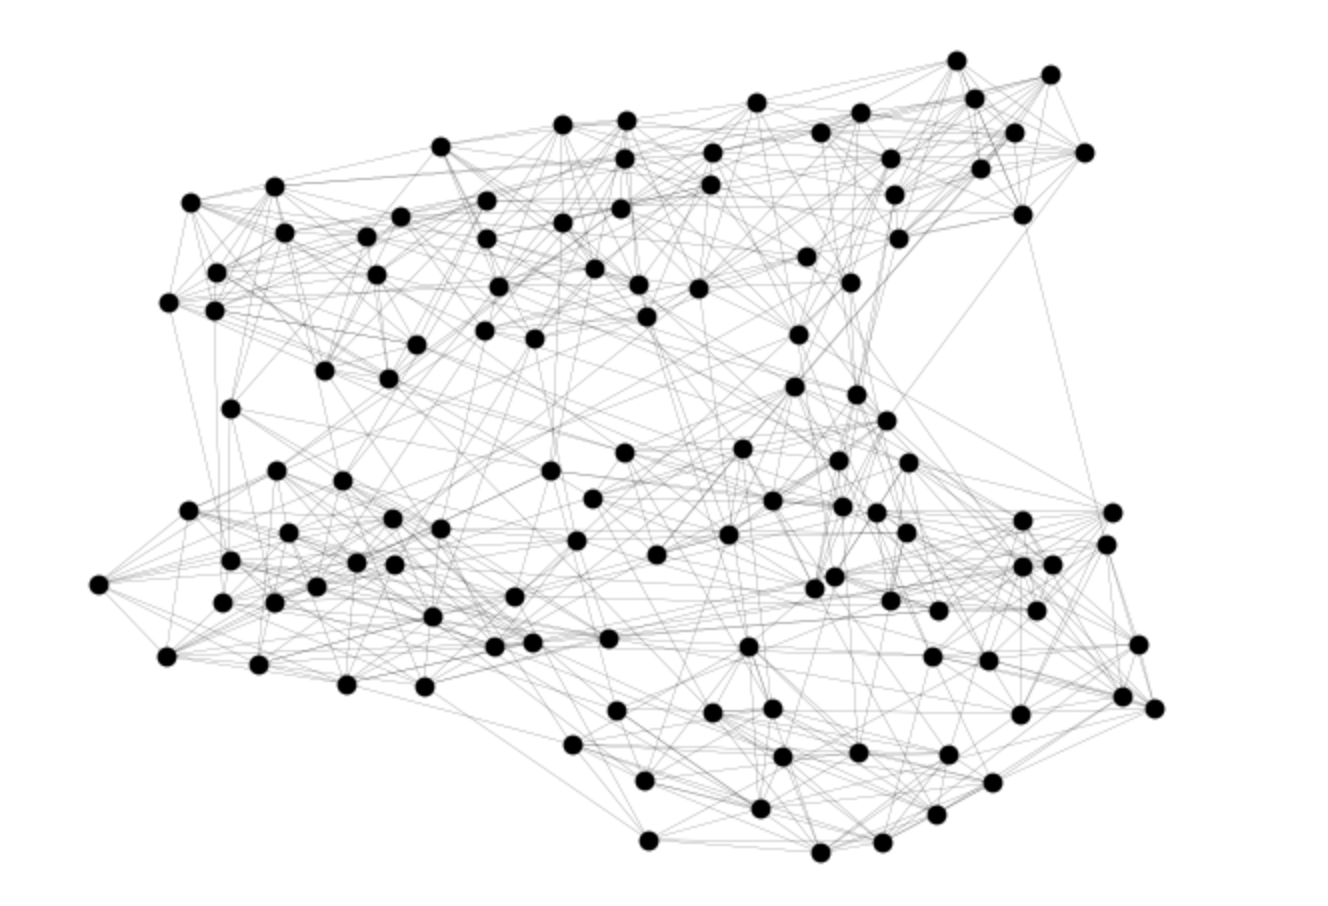
\includegraphics[scale=0.25]{american-football.png}
                    \end{figure}
                    \captionof{figure}{Clube de karatê de Zachary.}
                \end{minipage}
                \hfill
                \begin{minipage}[b]{0.49\textwidth}
                    \begin{figure}
                        \centering
                        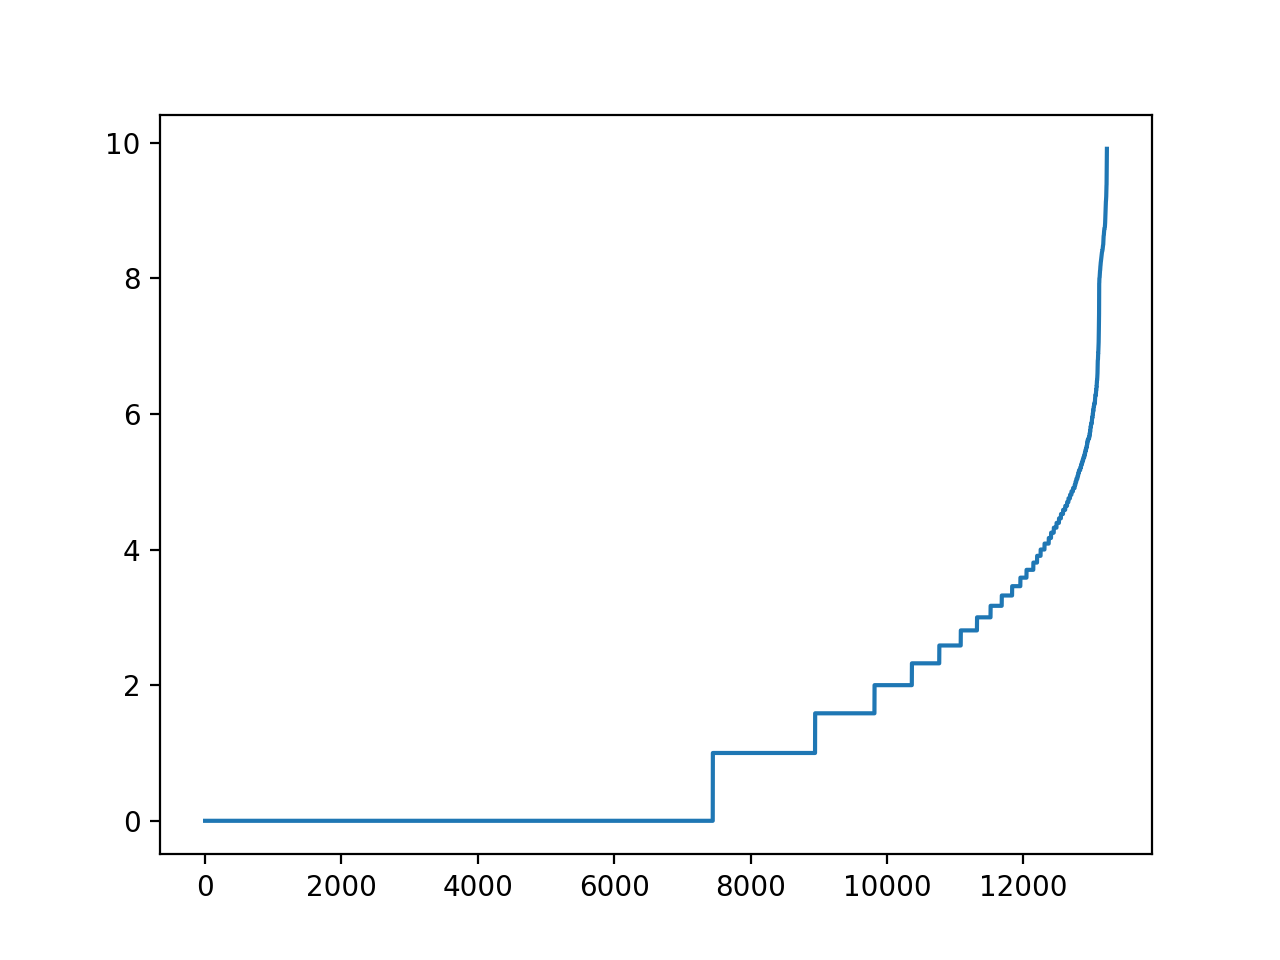
\includegraphics[scale=0.3]{short_path_centrality_ex3_log.png}
                    \end{figure}
                    \captionof{figure}{Representação gráfica.}
                \end{minipage}
            \end{minipage}
        \end{frame}

%----------------------------------------------------------------------------------------
%	Referências
%----------------------------------------------------------------------------------------
\section{Referências}
    \begin{frame}[t, allowframebreaks]
    \frametitle{Referências}
    \footnotesize{
        \begin{thebibliography}{99}
            \bibitem[]{} T. H. Cormen and C. E. Leiserson and R. L. Rivest and C. Stein (2009).
            \newblock Introduction to Algorithms.

            \bibitem[]{} D. Easley and J. Kleinberg (2010).
            \newblock Networks, Crowds, and Markets: Reasoning About a Highly Connected World
            \newblock https://www.cs.cornell.edu/home/kleinber/networks-book/networks-book.pdf.

            \bibitem[]{} Alane de Lima, Murilo da Silva and André Vignatti (2021).
            \newblock Shortest Path Centrality and the APSP problem via VC-dimension and Rademacher Averages.
            \newblock https://www.inf.ufpr.br/murilo/public/apsp-alg.pdf.
        \end{thebibliography}
    }
    \end{frame}
\end{document}